\chapter{Feature Request: Canvas Primitive \& Box Width Override}\label{record-016}

\noindent{\footnotesize\color{BookMuted}\path{docs/requests/xyph-title.md}\par}\smallskip

\textbf{From:} XYPH TUI title screen \textbf{Date:} 2026-02-28 \textbf{bijou version:} v0.9.0

\begin{center}\rule{0.5\linewidth}{0.5pt}\end{center}

\section{Context}\label{record-016-context}

XYPH's landing screen renders an animated ASCII spiral shader as a full-screen background, with the logo and status text inside a solid bordered box composited on top. With v0.9.0, \texttt{c\allowbreak{}o\allowbreak{}m\allowbreak{}p\allowbreak{}o\allowbreak{}s\allowbreak{}i\allowbreak{}t\allowbreak{}e\allowbreak{}(\allowbreak{})} + \texttt{b\allowbreak{}o\allowbreak{}x\allowbreak{}(\allowbreak{})} eliminate most of the hand-rolled compositing code, but two gaps remain.

\subsection{What v0.9.0 already solves}\label{record-016-what-v0.9.0-already-solves}

\begin{center}
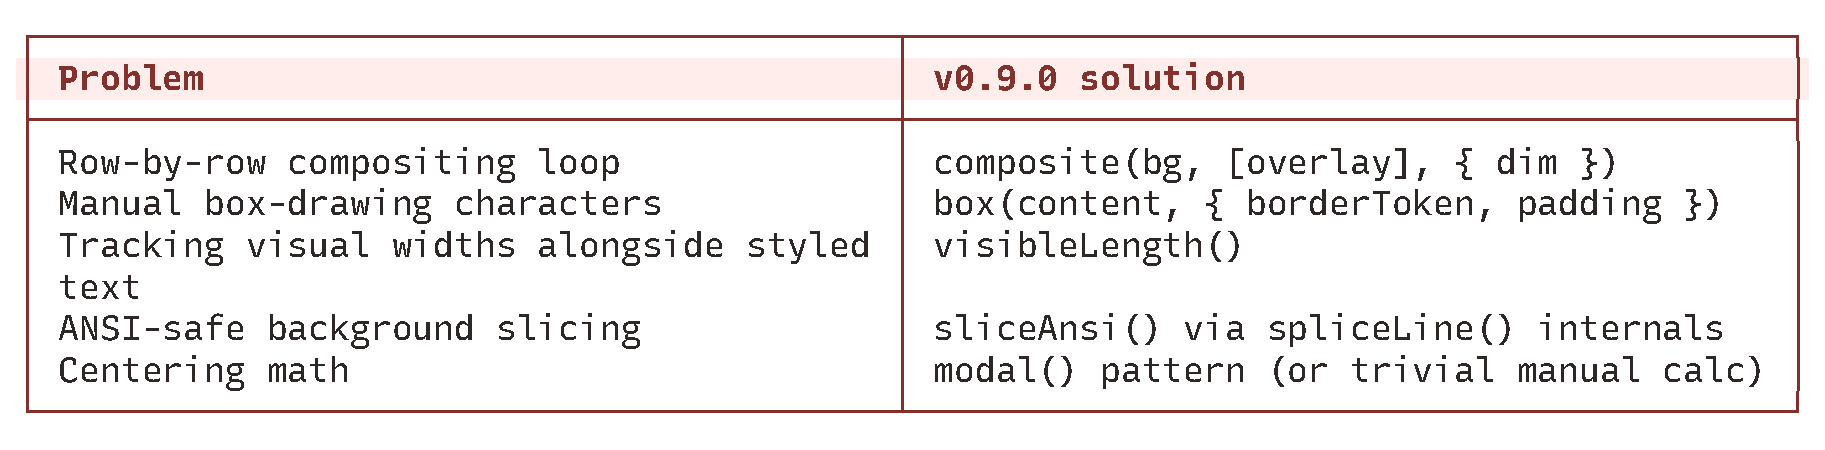
\includegraphics[width=\linewidth]{figures/tables/table-119-g1-1.pdf}
\par\smallskip{\scriptsize\color{BookMuted}Rows 1–5. Actual Bijou table component.}
\end{center}


\begin{center}\rule{0.5\linewidth}{0.5pt}\end{center}

\section{\texorpdfstring{Request 1: \texttt{c\allowbreak{}a\allowbreak{}n\allowbreak{}v\allowbreak{}a\allowbreak{}s\allowbreak{}(\allowbreak{})} --- Character-grid shader primitive}{Request 1:  --- Character-grid shader primitive}}\label{record-016-request-1-canvas-character-grid-shader-primitive}

\subsection{Problem}\label{record-016-problem}

The spiral background is a \texttt{(\allowbreak{}x\allowbreak{},\allowbreak{} \allowbreak{}y\allowbreak{},\allowbreak{} \allowbreak{}t\allowbreak{}i\allowbreak{}m\allowbreak{}e\allowbreak{})\allowbreak{} \allowbreak{}-\allowbreak{}>\allowbreak{} \allowbreak{}c\allowbreak{}h\allowbreak{}a\allowbreak{}r\allowbreak{}a\allowbreak{}c\allowbreak{}t\allowbreak{}e\allowbreak{}r} function evaluated over a \texttt{c\allowbreak{}o\allowbreak{}l\allowbreak{}s\allowbreak{} \allowbreak{}x\allowbreak{} \allowbreak{}r\allowbreak{}o\allowbreak{}w\allowbreak{}s} grid. The tight loop is pure boilerplate:

\begin{CodeBlock}
const lines: string[] = [];
for (let y = 0; y < rows; y++) {
  let line = '';
  for (let x = 0; x < cols; x++) {
    line += shaderFn(x, y, cols, rows, time);
  }
  lines.push(line);
}
return lines.join('\n');
\end{CodeBlock}

Every app that wants a procedural background (rain, static, plasma, matrix, starfield) re-implements this loop. The pattern is general enough to live in bijou.

\subsection{Proposed API}\label{record-016-proposed-api}

\begin{CodeBlock}
// bijou-tui or bijou core

type ShaderFn = (
  x: number,
  y: number,
  cols: number,
  rows: number,
  time: number,
) => string; // single character

function canvas(
  cols: number,
  rows: number,
  shader: ShaderFn,
  time?: number,
): string;
\end{CodeBlock}

\textbf{Returns:} A single string of \texttt{r\allowbreak{}o\allowbreak{}w\allowbreak{}s} newline-separated lines, each \texttt{c\allowbreak{}o\allowbreak{}l\allowbreak{}s} characters wide.

\textbf{Behavior:} - Calls \texttt{s\allowbreak{}h\allowbreak{}a\allowbreak{}d\allowbreak{}e\allowbreak{}r\allowbreak{}(\allowbreak{}x\allowbreak{},\allowbreak{} \allowbreak{}y\allowbreak{},\allowbreak{} \allowbreak{}c\allowbreak{}o\allowbreak{}l\allowbreak{}s\allowbreak{},\allowbreak{} \allowbreak{}r\allowbreak{}o\allowbreak{}w\allowbreak{}s\allowbreak{},\allowbreak{} \allowbreak{}t\allowbreak{}i\allowbreak{}m\allowbreak{}e\allowbreak{} \allowbreak{}?\allowbreak{}?\allowbreak{} \allowbreak{}0\allowbreak{})} for every cell - If the shader returns more than one character, take only the first - If it returns an empty string, substitute a space - \texttt{t\allowbreak{}i\allowbreak{}m\allowbreak{}e} defaults to \texttt{0} for static patterns

\subsection{Why bijou, not app code}\label{record-016-why-bijou-not-app-code}

\begin{enumerate}
\def\labelenumi{\arabic{enumi}.}
\tightlist
\item
  \textbf{Reusable} --- any TUI splash screen, screensaver, or background effect benefits from the same loop.
\item
  \textbf{Optimizable} --- bijou could later add row-level string building optimizations, canvas caching, or dirty-rect diffing without changing the shader contract.
\item
  \textbf{Composable} --- \texttt{c\allowbreak{}a\allowbreak{}n\allowbreak{}v\allowbreak{}a\allowbreak{}s\allowbreak{}(\allowbreak{})} output feeds directly into \texttt{c\allowbreak{}o\allowbreak{}m\allowbreak{}p\allowbreak{}o\allowbreak{}s\allowbreak{}i\allowbreak{}t\allowbreak{}e\allowbreak{}(\allowbreak{})} as a background string. The two together form a complete layered rendering pipeline.
\end{enumerate}

\subsection{Acceptance criteria}\label{record-016-acceptance-criteria}

\begin{CodeBlock}
canvas()
  ✓ calls shader(x, y, cols, rows, time) for every cell in order
  ✓ produces exactly `rows` lines separated by newlines
  ✓ each line is exactly `cols` characters wide
  ✓ truncates multi-char shader return to first character
  ✓ substitutes space for empty shader return
  ✓ time defaults to 0 when omitted
  ✓ works with cols=0 or rows=0 (returns empty string)
  pipe mode
    ✓ returns empty string (no visual output in pipes)
\end{CodeBlock}

\begin{center}\rule{0.5\linewidth}{0.5pt}\end{center}

\section{\texorpdfstring{Request 2: \texttt{b\allowbreak{}o\allowbreak{}x\allowbreak{}(\allowbreak{})} width override}{Request 2:  width override}}\label{record-016-request-2-box-width-override}

\subsection{Problem}\label{record-016-problem-1}

\texttt{m\allowbreak{}o\allowbreak{}d\allowbreak{}a\allowbreak{}l\allowbreak{}(\allowbreak{})} accepts an optional \texttt{w\allowbreak{}i\allowbreak{}d\allowbreak{}t\allowbreak{}h} to force a fixed box size, but \texttt{b\allowbreak{}o\allowbreak{}x\allowbreak{}(\allowbreak{})} doesn't. On the XYPH title screen, the box content changes between states:

\begin{center}
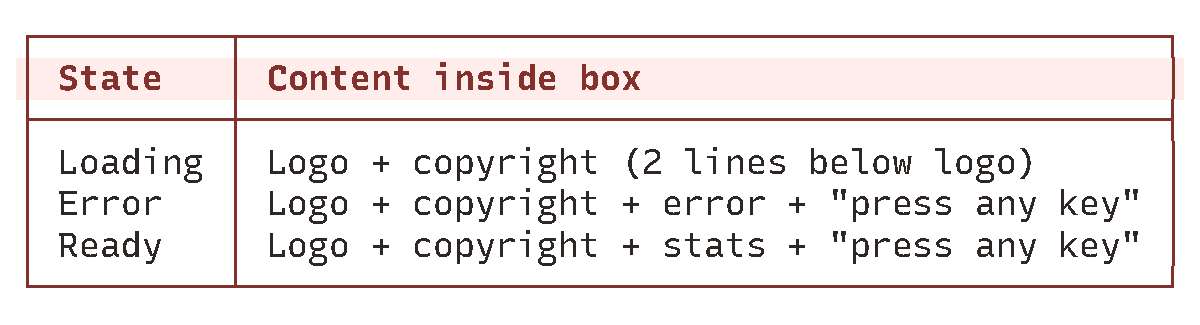
\includegraphics[width=\linewidth]{figures/tables/table-120-g1-1.pdf}
\par\smallskip{\scriptsize\color{BookMuted}Rows 1–3. Actual Bijou table component.}
\end{center}


The widest content line (the logo) is the same across all states, so the box width doesn't jump. But the box \emph{height} changes --- it's taller in the ready state than the loading state. If the widest line ever differed between states (e.g., a long error message), the box would visually jump widths between frames.

A \texttt{w\allowbreak{}i\allowbreak{}d\allowbreak{}t\allowbreak{}h} option on \texttt{b\allowbreak{}o\allowbreak{}x\allowbreak{}(\allowbreak{})} would let consumers lock the box to a fixed size for visual stability.

\subsection{Proposed API}\label{record-016-proposed-api-1}

\begin{CodeBlock}
export interface BoxOptions {
  borderToken?: TokenValue;
  padding?: { top?: number; bottom?: number; left?: number; right?: number };
  width?: number;  // <-- new: total outer width (border + padding + content)
  ctx?: BijouContext;
}
\end{CodeBlock}

\textbf{Behavior:} - When \texttt{w\allowbreak{}i\allowbreak{}d\allowbreak{}t\allowbreak{}h} is set, the box outer width is fixed to that value - Content lines shorter than the interior are right-padded with spaces - Content lines longer than the interior are clipped via \texttt{c\allowbreak{}l\allowbreak{}i\allowbreak{}p\allowbreak{}T\allowbreak{}o\allowbreak{}W\allowbreak{}i\allowbreak{}d\allowbreak{}t\allowbreak{}h\allowbreak{}(\allowbreak{})} - When \texttt{w\allowbreak{}i\allowbreak{}d\allowbreak{}t\allowbreak{}h} is not set, behavior is unchanged (auto-size to content)

\subsection{Acceptance criteria}\label{record-016-acceptance-criteria-1}

\begin{CodeBlock}
box() with width override
  ✓ outer width matches specified width exactly
  ✓ short content lines are right-padded to fill interior
  ✓ long content lines are clipped to interior width
  ✓ padding is subtracted from width to compute interior
  ✓ width < minimum (border + padding) produces zero-width interior
  ✓ visibleLength of every output line equals specified width
\end{CodeBlock}

\begin{center}\rule{0.5\linewidth}{0.5pt}\end{center}

\section{Non-request: Transparent compositing}\label{record-016-non-request-transparent-compositing}

Initially considered requesting a \texttt{t\allowbreak{}r\allowbreak{}a\allowbreak{}n\allowbreak{}s\allowbreak{}p\allowbreak{}a\allowbreak{}r\allowbreak{}e\allowbreak{}n\allowbreak{}t} option for \texttt{c\allowbreak{}o\allowbreak{}m\allowbreak{}p\allowbreak{}o\allowbreak{}s\allowbreak{}i\allowbreak{}t\allowbreak{}e\allowbreak{}(\allowbreak{})} where space characters in the overlay would reveal the background. After review, \texttt{c\allowbreak{}o\allowbreak{}m\allowbreak{}p\allowbreak{}o\allowbreak{}s\allowbreak{}i\allowbreak{}t\allowbreak{}e\allowbreak{}(\allowbreak{})}'s current opaque behavior is correct for the box use case --- the solid interior is the whole point. Transparent compositing is a different primitive (sprite rendering) and would complicate the common case. Noting it here as a future thought, not a request.

\begin{center}\rule{0.5\linewidth}{0.5pt}\end{center}

\section{Usage sketch (v0.9.0 + these two features)}\label{record-016-usage-sketch-v0.9.0-these-two-features}

\begin{CodeBlock}
import { box } from '@flyingrobots/bijou';
import { composite, canvas } from '@flyingrobots/bijou-tui';
import { spiralShader } from './shaders/spiral.js';

export function landingView(model: DashboardModel): string {
  // 1. Render full-screen spiral background
  const bg = canvas(model.cols, model.rows, spiralShader, Date.now());
  const styledBg = styled(muted, bg);

  // 2. Build foreground content
  const content = [gradientLogo, '', copyright, '', statusText]
    .filter(Boolean).join('\n');

  // 3. Wrap in a fixed-width box
  const panel = box(content, {
    borderToken: border,
    padding: { top: 1, bottom: 1, left: 3, right: 3 },
    width: logoWidth + 8, // lock to logo width + padding + border
  });

  // 4. Center and composite
  const panelLines = panel.split('\n');
  const row = Math.floor((model.rows - panelLines.length) / 2);
  const col = Math.floor((model.cols - visibleLength(panelLines[0])) / 2);

  let result = composite(styledBg, [{ content: panel, row, col }], { dim: true });

  // 5. Progress bar at bottom
  if (model.loading) {
    const bar = progressBar(model.loadingProgress, { width: model.cols });
    result = composite(result, [{ content: bar, row: model.rows - 1, col: 0 }]);
  }

  return result;
}
\end{CodeBlock}

\textasciitilde25 lines vs.~the current \textasciitilde130 lines of manual compositing.

